\section{字句解析}
\subsection{字句解析}

\begin{figure}[H]
  \centering
  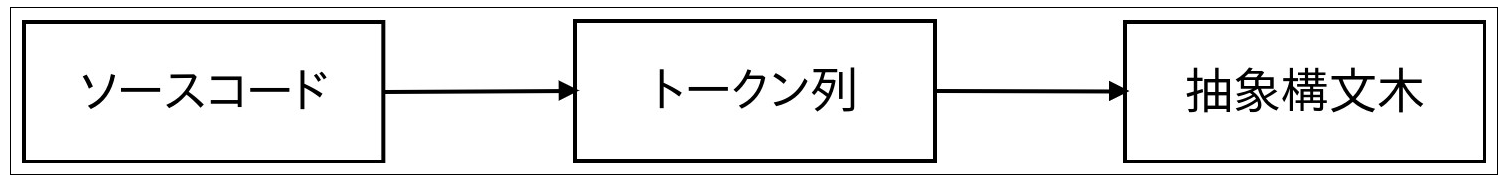
\includegraphics[height=2.0cm]{fig/fig1-1.png}
  \caption{ソースコードの他の形式への変更}
  \label{fig:1}
\end{figure}

字句解析: ソースコードからトークン列への変換

字句解析器: トークナイザー,スキャナー

トークン列: 小さな,分類しやすいデータ構造,あとで構文解析器に渡される

\begin{lstlisting}[caption=入力の例1]
let x = 5 + 5;
\end{lstlisting}

\begin{lstlisting}[caption=出力の例1]
[
  LET,
  IDENTIFIER("x"),
  EQUAL_SIGN,
  INTEGER(5),
  PLUS_SIGN,
  INTEGER(5),
  SEMICOLON
]
\end{lstlisting}

\subsection{トークンを定義する}

\begin{lstlisting}[caption=Monkey言語の例]
let five = 5;
let ten = 10;

let add = fn(x, y) {
  x + y;
}

let result = add(five, ten);
\end{lstlisting}

\subsection{字句解析器(レキサー)}

字句解析器: ソースコードを入力として受け取り,出力としてそのソースコードを表現するトークン列を返す

字句解析器は入力を先頭から読み進み,認識したトークンを順に一つずつ出力する

\subsection{トークン集合の拡充と字句解析器の拡張}

\subsection{REPLの始まり}

REPL: コンソールやインタラクティブモードと呼ばれることもある
